In this chapter experiments with real servos will be conducted in order to, firstly, tune the parameters of the simulation (servo's characteristics) and, secondly, verify that the simulation correctly predicts the behaviour of a real-life configuration.

\section{Experimental set-up}
The set-up is explained on \cref{fig:exp_setup}. In later experiments a camera will be used to film the motion of the servos and compare it to the results of the simulation that is supposed to predict it.

\begin{figure}[htp]
\center
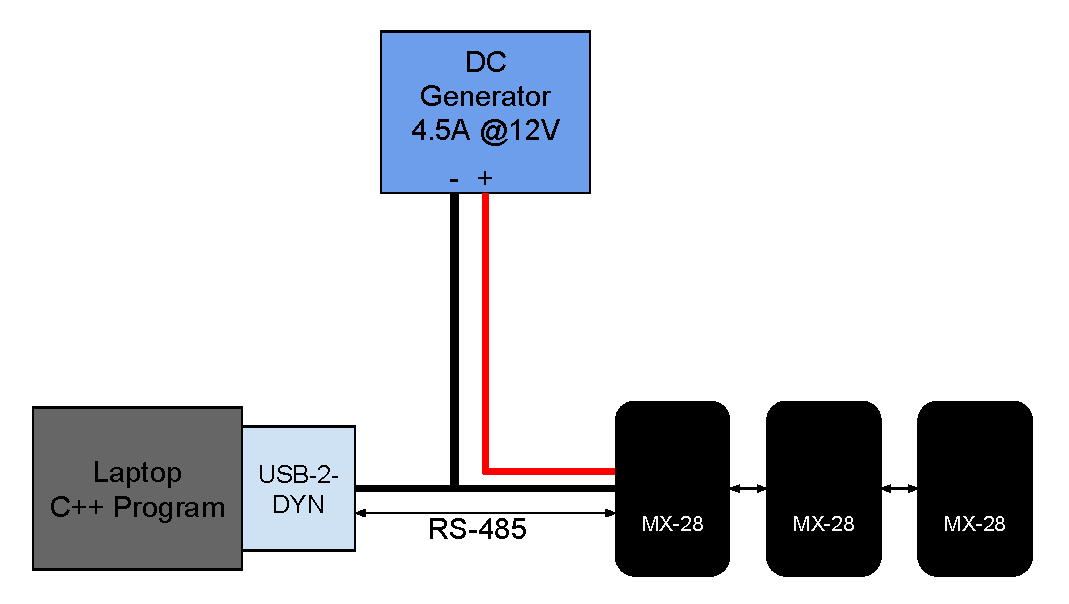
\includegraphics[width=0.6\textwidth]{figures/exp_setup}
\caption{Experimental setup : The MX-28 servos are powered by a DC generator and controlled by a laptop equipped with a USB2DYNAMIXEL(USB-2-DYN) device. It converts an USB port into a serial port.}
\label{fig:exp_setup}
\end{figure}

\section{Experiments}
The purpose of the first experiment is to test the torque : to that end, a frame is fixed onto a single servo and weighted. The setup is represented on \cref{fig:exp1}.

At $12V$, the maximal torque of the servo is supposedly $2.5N.m$, as claimed by \cite{mx_28_manual}. To test this, a weight of $2kg$ is hanged at $12.5cm$ from the center of the servo, because since 
\begin{align*}
2.5 - 9.81 \cdot (0.007 \cdot 0.01 + 0.016 \cdot 0.0725) &= x \cdot 0.125\\
x &= 20 N\\
&= 2.03 kg
\end{align*}

\begin{figure}[htp]
\center
    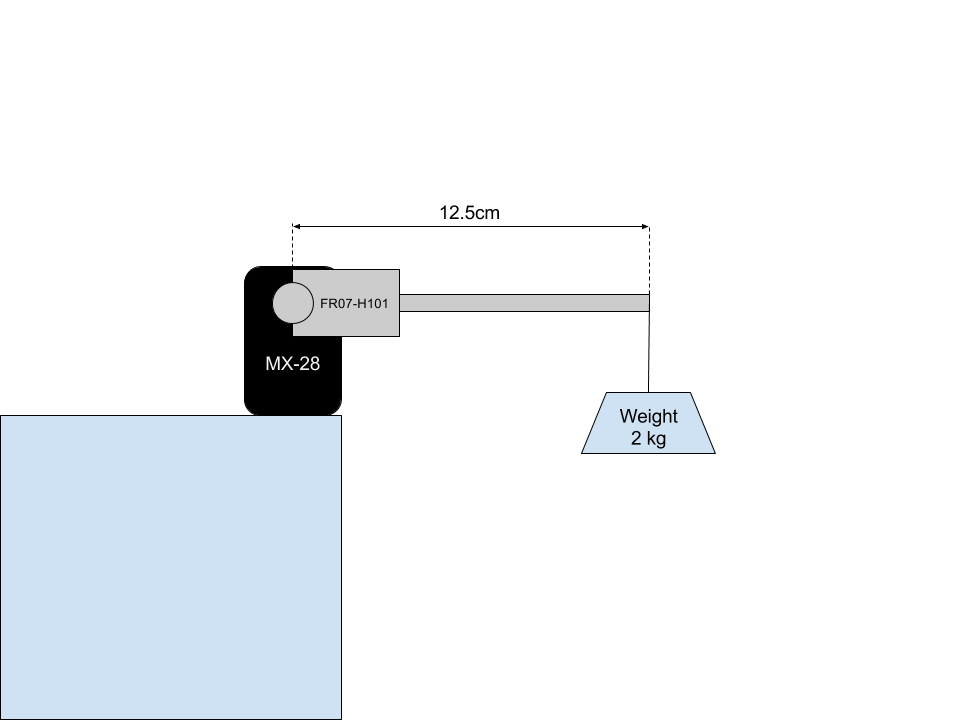
\includegraphics[width = 0.5\textwidth]{figures/exp1}
    \caption[Experimental setup for torque testing]{Experimental setup for torque testing : A weight of $2kg$ is suspended at $12.5cm$ from the servo, resulting in a torque of $2.5Nm$. The goal is to test whether the servo is able to move the weight upwards from the depicted initial situation.}
    \label{fig:exp1}
\end{figure}

The experimental results are compared to the claims of \cite{mx_28_manual} in \cref{table:exp1_results}.
\begin{table}[htp]
\center
\begin{tabularx}{\textwidth}{@{}l X X X @{}}
\toprule
& \textbf{Stall torque @11.1V $[N.m]$} & \textbf{Stall torque @12V $[N.m]$} & \textbf{Stall torque @14.8V $[N.m]$}\\ 
\midrule
\textbf{Theoretical} & 2.1 & 2.5 & 3.1\\ 
\textbf{Experimental} &  &  & \\ 
\bottomrule
\end{tabularx}
\caption{Experimental stall torques at different tested voltages}
\label{table:exp1_results}
\end{table}

\section{Servo tuning}

\section{Results}